% Provenance (never printed): see sources/outline_sources.md (Year 3:
% geomorphology, hillslope processes, river incision, landscape evolution).
% Brief: sources/book5/BRIEFS.md, ch. 18. Curves from
% figdata/bachelor-3/hillslope.py, stream_profile.py and varden_river.py.
% Exercise and problem values in the Book 5 scratch calculator calc/ch18.py.
% The upland west of the Varden Hills, its river, its tributaries, its
% uplift rate and its base-level fall are invented; the outlet elevation is
% the region model's river at the west edge of the map.
\chapter{Geomorfología cuantitativa}\label{ch:b3:quantitative-geomorphology}

Un río que atraviesa una cordillera en ascenso presenta un escalón en su perfil longitudinal: una cascada,
con un desfiladero aguas abajo y un valle más suave aguas arriba. El escalón no permanece
donde se formó. Remonta aguas arriba, a razón de unos pocos milímetros o unos pocos metros al
año, y su posición es un reloj que se puso en marcha cuando el \omterm{def:b3:quantitative-geomorphology:knickpoint}{nivel de base} del río
fue rebajado. Leer ese reloj, y las tasas escritas en la forma de las laderas
y los ríos, requiere dos leyes de conservación y dos leyes de transporte: una para el
suelo que se desliza lentamente ladera abajo, y otra para el lecho rocoso que corta el río.

\begin{recall}
La meteorización, la erosión, la sedimentación, las formas del relieve y el equilibrio entre levantamiento
y erosión figuran en los libros de niveles anteriores, al igual que el rebote isostático y los
valles glaciares en U. La tasa de denudación, el esfuerzo de cizalla en el lecho y el parámetro de Shields
figuran en el volumen de primer año, en su capítulo sobre erosión y transporte;
el modelo digital de elevaciones en su capítulo sobre mapas geológicos; la
isostasia de Airy en su capítulo sobre isostasia y anomalías gravimétricas. Los
\omterm{def:b3:advanced-geochronology:cosmogenic}{nucleidos cosmogénicos} y las tasas de erosión obtenidas a partir de ellos están en
el capítulo~\ref{ch:b3:advanced-geochronology}, la \omterm{def:b3:orogenic-wedges:thermochronology}{termocronología} y la
\omterm{def:b3:orogenic-wedges:age-elevation}{relación edad--altitud} en el capítulo~\ref{ch:b3:orogenic-wedges}. La
ecuación de difusión figura en los libros de física.
\end{recall}

\section{Laderas}\label{sec:b3:quantitative-geomorphology:hillslopes}

En una colina cubierta de suelo, este se desplaza ladera abajo grano a grano: los animales excavadores lo remueven,
las raíces lo levantan, la congelación y la humectación lo hinchan, y cada
perturbación permite que la gravedad lo desplace un poco. Promediado a lo largo de siglos, el
flujo de suelo es proporcional a la pendiente.

\begin{definition}[Difusión de laderas]\label{def:b3:quantitative-geomorphology:diffusion}
La \emph{difusión de laderas}\index{difusión de laderas} es el lento
transporte de suelo ladera abajo cuyo flujo volumétrico por unidad de ancho de ladera,
$\vec q$, es proporcional al gradiente de la elevación superficial $z$:
$\vec q = -\kappa\,\nabla z$. El coeficiente $\kappa$, en
\unit{m^2/yr}, es la difusividad de ladera.
\end{definition}

\begin{theorem}[Difusión de laderas]\label{thm:b3:quantitative-geomorphology:diffusion}
Sea la roca levantada a una tasa $U$ con respecto a los cauces que delimitan una
ladera, el suelo y la roca tienen la misma densidad, y el suelo se mueve por \omterm{def:b3:quantitative-geomorphology:diffusion}{difusión de laderas}
con $\kappa$ uniforme. Entonces la elevación superficial obedece
\[
\frac{\partial z}{\partial t} = U + \kappa\,\nabla^2 z ,
\]
la ecuación de difusión con un término fuente.
\end{theorem}

\begin{proof}
Se toma un área pequeña $\delta S$ de la ladera. Su volumen cambia por el levantamiento,
$U\,\delta S$ por unidad de tiempo, y por el suelo que sale a través de sus
bordes, $\oint \vec q\cdot\vec n\,\mathrm{d}\ell = (\nabla\cdot\vec q)\,\delta S$.
Por tanto, $\partial z/\partial t = U - \nabla\cdot\vec q$; con $\vec q = -\kappa
\nabla z$ y $\kappa$ uniforme, $\nabla\cdot\vec q = -\kappa\nabla^2 z$.
\end{proof}

Una falla o una línea de costa cortan un escarpe en un instante; después, el escarpe solo
evoluciona por difusión. Partiendo de un escalón vertical de semialtura $a$ sobre una
pendiente de campo lejano $b$, la solución en una dimensión es
\[
z(x,t) = a\,\operatorname{erf}\!\left(\frac{x}{2\sqrt{\kappa t}}\right) + b\,x ,
\qquad
\left.\frac{\partial z}{\partial x}\right|_{x=0} = \frac{a}{\sqrt{\pi\kappa t}} + b .
\]
La forma depende solo del producto $\kappa t$: un perfil medido permite obtener
$\kappa t$; o bien una edad independiente da $\kappa$, o bien
un $\kappa$ conocido da la edad, una \emph{edad morfológica}. Los escarpes en regiones semiáridas
con suelos granulares y vegetación escasa dan valores de $\kappa$ entre
$10^{-3}$ y \qty{e-2}{m^2/yr}; en las montañas costeras húmedas y densamente
vegetadas, alrededor de \qty{5e-3}{m^2/yr}.
% ledger: whipple04:scarp-erf, whipple04:scarp-kappa

\begin{omfigure}
\begin{tikzpicture}
\begin{groupplot}[group style={group size=2 by 1, horizontal sep=1.6cm},
  width=0.48\linewidth, height=0.36\linewidth, tick label style={font=\scriptsize},
  label style={font=\small}, legend style={font=\scriptsize, draw=none, fill=none}]
\nextgroupplot[xlabel={distancia $x$ (m)}, ylabel={$z$ (m)}, xmin=-40, xmax=40,
  ymin=-5, ymax=5, legend pos=north west]
% computed in figdata/bachelor-3/hillslope.py
\addplot[black!50, densely dashed] table[x=x, y=z0] {figdata/out/bachelor-3-hillslope-scarp.dat};
\addplot[omDef, thick] table[x=x, y=z1] {figdata/out/bachelor-3-hillslope-scarp.dat};
\addplot[omProp, thick] table[x=x, y=z2] {figdata/out/bachelor-3-hillslope-scarp.dat};
\addplot[omThm, thick] table[x=x, y=z3] {figdata/out/bachelor-3-hillslope-scarp.dat};
\legend{inicial, \qty{2}{kyr}, \qty{10}{kyr}, \qty{40}{kyr}}
\nextgroupplot[xlabel={distancia a la divisoria (m)}, ylabel={altura (m)},
  xmin=-150, xmax=150, ymin=0, ymax=200, xtick={-150,-75,0,75,150}]
\addplot[omMeth, thick] table[x=x, y=z1] {figdata/out/bachelor-3-hillslope-hill.dat};
\addplot[omDef, thick] table[x=x, y=z2] {figdata/out/bachelor-3-hillslope-hill.dat};
\addplot[omThm, thick] table[x=x, y=z3] {figdata/out/bachelor-3-hillslope-hill.dat};
\node[font=\scriptsize, anchor=north] at (axis cs:0,45) {0.0215};
\node[font=\scriptsize, anchor=north] at (axis cs:0,94) {0.043};
\node[font=\scriptsize, anchor=north] at (axis cs:0,184) {\qty{0.086}{mm/yr}};
\end{groupplot}
\end{tikzpicture}

\par\smallskip{\small Izquierda, un escarpe de \qty{5}{m} de desplazamiento en una pendiente de
0.05, que se difunde con $\kappa = \qty{5e-3}{m^2/yr}$: el escalón inicial
(a trazos) y los perfiles tras 2, 10 y \qty{40}{kyr}. Derecha, colinas
estacionarias de semianchura \qty{150}{m} con el mismo $\kappa$ (altura sobre los
cauces), que descienden a
0.0215, 0.043 y \qty{0.086}{mm/yr}: parábolas cuyo relieve y curvatura de la cima
son proporcionales a la tasa de erosión.}\label{fig:b3:quantitative-geomorphology:hillslope}
\end{omfigure}
% ledger: whipple04:scarp-kappa

Cuando una colina se ha levantado y erosionado durante el tiempo suficiente, su forma deja de cambiar:
cada punto desciende a la misma velocidad a la que asciende la roca.

\begin{proposition}[La curvatura de la cima mide la tasa de erosión]\label{prop:b3:quantitative-geomorphology:curvature}
En una ladera en \omterm{def:b3:quantitative-geomorphology:steady-profile}{estado estacionario} bajo difusión de ladera, la tasa de erosión
$E$, igual a $U$, es
\[
E = -\kappa\,\nabla^2 z .
\]
En una dimensión, el perfil es la parábola $z = z_0 - E x^2/(2\kappa)$,
con un relieve $E L^2/(2\kappa)$ entre la divisoria y los cauces, situados a una distancia
$L$.
\end{proposition}

\begin{proof}
Imponiendo $\partial z/\partial t = 0$ en el teorema se obtiene $\kappa\nabla^2 z =
-U = -E$. En una dimensión, dos integraciones con $\mathrm{d}z/\mathrm{d}x =
0$ en la divisoria dan la parábola, y su valor en $x = L$ da el relieve.
\end{proof}

La curvatura, magnitud geométrica medida sobre un modelo digital de elevaciones, se interpreta así
como una tasa una vez conocido $\kappa$: cuanto más empinadas y más agudamente redondeadas
sean las cimas, más deprisa se erosiona el paisaje. El propio suelo se forma a partir de
la roca subyacente, a una tasa que depende de cuánto suelo ya la cubre.

\begin{definition}[Función de producción de suelo]\label{def:b3:quantitative-geomorphology:soil-production}
La \emph{función de producción de suelo}\index{función de producción de suelo} proporciona
la tasa $P$ a la que el lecho rocoso se convierte en suelo en función del
espesor del suelo $h$; habitualmente se toma $P = P_0\,e^{-h/h_0}$, donde
$P_0$ es la tasa sobre roca desnuda y $h_0$ una longitud de una fracción de metro.
\end{definition}

En \omterm{def:b3:quantitative-geomorphology:steady-profile}{estado estacionario}, la interfase suelo-roca desciende a la tasa de la
superficie, $P(h) = E$, de modo que el espesor del suelo es $h = h_0 \ln(P_0/E)$: una
erosión más rápida implica un suelo más delgado, y donde $E$ supera a $P_0$ el suelo
se elimina y aflora la roca desnuda, limitada por la meteorización. Las tasas de producción de suelo
más rápidas medidas son del orden de \qty{0.5}{mm/yr}.
% ledger: whipple04:soil

La difusión lineal falla en pendientes pronunciadas. A medida que el gradiente se acerca a un
umbral, los granos ruedan y deslizan en ráfagas y los deslizamientos someros eliminan el
suelo.

\begin{definition}[Pendiente crítica de ladera]\label{def:b3:quantitative-geomorphology:critical}
La \emph{pendiente crítica de ladera}\index{pendiente crítica de ladera}
$S_c$ es el gradiente al que el flujo de suelo crece sin límite; en una ley de transporte no lineal
muy utilizada, $q = \kappa S/[1 - (S/S_c)^2]$.
\end{definition}

Las pendientes mucho más suaves que $S_c$ se comportan como en la difusión lineal; las pendientes
que se erosionan deprisa se empinan hacia $S_c$ y se vuelven planas, con un gradiente fijado
por el umbral y no por la tasa de erosión.
% ledger: whipple04:nonlinear

\begin{inthefield}[Escaneado de una ladera]
Un equipo que estudia una loma cubierta de suelo coloca un escáner láser terrestre sobre un
trípode a unas decenas de metros de la cresta. Cada escaneo registra millones de
puntos, la distancia y la dirección hasta la superficie del terreno, a través de los huecos
entre la hierba y los arbustos; los puntos de varias estaciones de escaneo se fusionan
en una única nube, registrada con dianas topográficas mediante un receptor de satélite,
y se conservan los últimos retornos para eliminar la vegetación. La nube del suelo desnudo
se transforma en una malla de elevaciones de celdas decimétricas, suavizada a lo largo de unos
metros, y su laplaciano se calcula en la cresta. El equipo compara después las
curvaturas de las cimas de las lomas que se erosionan a tasas medidas con \omterm{def:b3:advanced-geochronology:cosmogenic}{nucleidos
cosmogénicos}: representadas una frente a otra, las dos dan la difusividad de la
ladera como pendiente de una recta, tal como predice la proposición.
\end{inthefield}

\section{Incisión fluvial}\label{sec:b3:quantitative-geomorphology:rivers}

Donde un río discurre sobre lecho rocoso, se encaja mediante el arranque de bloques, por
abrasión bajo su carga de fondo y por cavitación. Todos estos procesos escalan con el esfuerzo
de cizalla que el flujo ejerce sobre su lecho, o con la potencia que disipa allí, y ambos crecen
con el caudal y la pendiente. El caudal crece con el área de drenaje, de modo que el área
representa al caudal.

\begin{definition}[Ley de potencia de la corriente]\label{def:b3:quantitative-geomorphology:stream-power}
La \emph{ley de potencia de la corriente}\index{ley de potencia de la corriente} proporciona la tasa
de incisión vertical $E$ de un río sobre lecho rocoso, como
\[
E = K A^m S^n ,
\]
donde $A$ es el área de drenaje aguas arriba del punto, $S$ la pendiente del cauce, $m$ y $n$
exponentes positivos, y $K$ un coeficiente de erosionabilidad que agrupa la resistencia de la roca,
el clima y la anchura del cauce.
\end{definition}

Para los procesos que escalan con el esfuerzo de cizalla o con la potencia unitaria de la corriente,
$m/n$ está próximo a 0.5. Un estudio de cauces de cárcavas excavados en roca débil durante
unos 20 años encontró tasas de incisión proporcionales a $A^{0.44}S^{0.68}$.
% ledger: whipple04:spim

\begin{definition}[Incisión limitada por el arranque y limitada por el transporte]\label{def:b3:quantitative-geomorphology:limited}
La incisión es \emph{limitada por el arranque}\index{incisión limitada por el arranque} cuando el río puede
transportar más sedimento del que recibe, de modo que su tasa de descenso se fija por la rapidez
con que arranca el lecho rocoso de su cauce: en ese caso se aplica la
\omterm{def:b3:quantitative-geomorphology:stream-power}{ley de potencia de la corriente}. Es
\emph{limitada por el transporte}\index{incisión limitada por el transporte} cuando el río
transporta todo el sedimento que puede, de modo que su lecho solo desciende donde la capacidad
de transporte aumenta aguas abajo, a la tasa fijada por la divergencia
del flujo de sedimento.
\end{definition}

Un río \omterm{def:b3:quantitative-geomorphology:limited}{limitado por el transporte} se comporta de forma muy parecida a una ladera: el flujo
depende de la pendiente, y su perfil evoluciona mediante una ecuación de tipo difusivo que
redondea cualquier escalón. Un río \omterm{def:b3:quantitative-geomorphology:limited}{limitado por el arranque} mantiene un escalón agudo y lo
desplaza, como muestra la siguiente sección. Los ríos de montaña con lecho rocoso y gravas
delgadas suelen parecerse más al primero; los ríos sobre aluviones gruesos, al
segundo.

\begin{omfigure}
\begin{tikzpicture}[x=0.55cm, y=0.55cm, font=\scriptsize,
  declare function={f(\x)=2.1+3.5*(1-(\x-0.5)/10)^2;
    tl(\x,\l)=f(\x)-1.1*exp(-(10.5-\x)/\l);}]
\begin{scope}
\draw[->] (0,0) -- (11.5,0) node[below left] {distancia aguas abajo};
\draw[->] (0,0) -- (0,6) node[above right] {$z$};
\draw[black!50, densely dashed] plot[domain=0.5:10.5, samples=40] (\x,{f(\x)});
\draw[omDef, thick] plot[domain=0.5:6.5, samples=30] (\x,{f(\x)}) -- plot[domain=6.5:10.5, samples=20] (\x,{f(\x)-1.1});
\draw[omThm, thick] plot[domain=0.5:3.5, samples=20] (\x,{f(\x)}) -- plot[domain=3.5:10.5, samples=30] (\x,{f(\x)-1.1});
\draw[->, black!70] (6.3,4.1) -- (3.8,4.75);
\node[anchor=west, align=left] at (5.6,5.3) {limitado por el arranque:\\ el escalón se desplaza aguas arriba};
\node at (5.5,-0.7) {(a)};
\end{scope}
\begin{scope}[xshift=7.2cm]
\draw[->] (0,0) -- (11.5,0) node[below left] {distancia aguas abajo};
\draw[->] (0,0) -- (0,6) node[above right] {$z$};
\draw[black!50, densely dashed] plot[domain=0.5:10.5, samples=40] (\x,{f(\x)});
\draw[omDef, thick] plot[domain=0.5:10.5, samples=40] (\x,{tl(\x,1.2)});
\draw[omThm, thick] plot[domain=0.5:10.5, samples=40] (\x,{tl(\x,3.5)});
\node[anchor=west, align=left] at (5.0,5.3) {limitado por el transporte:\\ el descenso se difunde aguas arriba};
\node at (5.5,-0.7) {(b)};
\end{scope}
\end{tikzpicture}

\par\smallskip{\small La respuesta de un río a un descenso de su \omterm{def:b3:quantitative-geomorphology:knickpoint}{nivel de base}
(en trazo discontinuo: el perfil antes del descenso; en azul, y después en rojo: dos instantes posteriores),
esquemática. (a) Un río \omterm{def:b3:quantitative-geomorphology:limited}{limitado por el arranque} conserva un \omterm{def:b3:quantitative-geomorphology:knickpoint}{punto de ruptura de pendiente} agudo que
migra aguas arriba; aguas abajo de él, el perfil conserva su forma antigua, rebajada. (b) Un río
\omterm{def:b3:quantitative-geomorphology:limited}{limitado por el transporte} rebaja todo su perfil de forma progresiva, sobre todo cerca de la
desembocadura.}\label{fig:b3:quantitative-geomorphology:regimes}
\end{omfigure}

Si la roca asciende a una tasa uniforme $U$ respecto a la desembocadura del río, y $K$,
$m$, $n$ son uniformes, el río evoluciona según $\partial z/\partial t = U - K A^m
S^n$.

\begin{definition}[Perfil en estado estacionario]\label{def:b3:quantitative-geomorphology:steady-profile}
Un perfil fluvial está en \emph{estado estacionario}\index{estado estacionario}
cuando su elevación ya no cambia con el tiempo: en cada punto, la incisión
compensa el levantamiento de la roca respecto a la desembocadura.
\end{definition}

\begin{theorem}[Perfil en estado estacionario bajo la ley de potencia de la corriente]\label{thm:b3:quantitative-geomorphology:steady}
Con $U$, $K$, $m$ y $n$ uniformes, un río \omterm{def:b3:quantitative-geomorphology:limited}{limitado por el arranque} en \omterm{def:b3:quantitative-geomorphology:steady-profile}{estado
estacionario} tiene la pendiente
\[
S = \left(\frac{U}{K}\right)^{1/n} A^{-m/n} .
\]
\end{theorem}

\begin{proof}
En el \omterm{def:b3:quantitative-geomorphology:steady-profile}{estado estacionario} $\partial z/\partial t = 0$, así que $K A^m S^n = U$, de donde $S^n
= (U/K)A^{-m}$; tomando la raíz $n$-ésima se obtiene el resultado.
\end{proof}

\begin{omfigure}
\begin{tikzpicture}
\begin{groupplot}[group style={group size=2 by 1, horizontal sep=1.7cm},
  width=0.48\linewidth, height=0.33\linewidth, tick label style={font=\scriptsize},
  label style={font=\small}]
\nextgroupplot[xlabel={distancia desde la divisoria (km)}, ylabel={$z$ (m)},
  xmin=0, xmax=12, ymin=150, ymax=420]
% computed in figdata/bachelor-3/stream_profile.py
\addplot[omDef, thick] table[x=d, y=z] {figdata/out/bachelor-3-stream_profile-steady.dat};
\nextgroupplot[xmode=log, ymode=log, xlabel={área de drenaje $A$ (\unit{km^2})},
  ylabel={pendiente $S$}, xmin=0.1, xmax=100, ymin=0.003, ymax=0.2]
\addplot[omDef, thick] table[x=A, y=S] {figdata/out/bachelor-3-stream_profile-steady.dat};
\addplot[only marks, mark=*, mark size=1.4pt, omThm] table[x=A, y=S] {figdata/out/bachelor-3-stream_profile-sa.dat};
\addplot[omThm, densely dashed] table[x=A, y=S] {figdata/out/bachelor-3-stream_profile-fit.dat};
\end{groupplot}
\end{tikzpicture}

\par\smallskip{\small El perfil en \omterm{def:b3:quantitative-geomorphology:steady-profile}{estado estacionario} del río de montaña ficticio
al oeste de las colinas de Varden ($U = \qty{0.043}{mm/yr}$, $K =
\qty{e-6}{yr^{-1}}$, $m = 0.5$, $n = 1$), desde su cabecera hasta la
desembocadura a \qty{170}{m}. A la derecha, pendiente frente a área: el modelo (línea
azul) y doce pendientes medidas en tramos de \qty{200}{m} con una dispersión de unos
\qty{10}{\percent} (puntos rojos), cuya recta de mínimos cuadrados
(discontinua) tiene una pendiente de $-0.47$.}\label{fig:b3:quantitative-geomorphology:profile}
\end{omfigure}

La pendiente disminuye como potencia del área: el perfil es cóncavo hacia arriba. Los ríos reales
siguen una ley de potencia de este tipo incluso cuando las hipótesis del teorema son dudosas, de modo que
dos números resumen un perfil.
% ledger: whipple04:steepness

\begin{definition}[Índices de pendiente del cauce y de concavidad]\label{def:b3:quantitative-geomorphology:indices}
Cuando la pendiente de un río sigue $S = k_s A^{-\theta}$, el exponente
$\theta$ es el \emph{índice de concavidad}\index{índice de concavidad} y el
coeficiente $k_s$ el \emph{índice de pendiente del cauce}\index{índice de pendiente del cauce}.
Para comparar ríos, $\theta$ se fija en un valor de referencia común
$\theta_{\mathrm{ref}}$, y $k_{sn} = S A^{\theta_{\mathrm{ref}}}$ es la
pendiente normalizada.
\end{definition}

Según el teorema, $\theta = m/n$ y $k_s = (U/K)^{1/n}$: con una erodibilidad dada, un río es más
empinado donde la roca asciende más deprisa. Los mapas de pendiente de una cordillera delinean,
por tanto, su levantamiento.


Las pendientes son derivadas de elevaciones con ruido y se dispersan mucho. Integrar
el perfil, en cambio, usa elevaciones, que se miden con más precisión.

\begin{definition}[Análisis chi]\label{def:b3:quantitative-geomorphology:chi}
El \emph{análisis chi}\index{análisis chi} representa la elevación de los puntos
de una red fluvial frente a la coordenada
\[
\chi(x) = \int_{x_b}^{x} \left(\frac{A_0}{A(x')}\right)^{\theta}
\mathrm{d}x' ,
\]
donde $x$ es la distancia aguas arriba a lo largo del cauce desde un punto base
$x_b$, $A_0$ un área de referencia y $\theta$ el \omterm{def:b3:quantitative-geomorphology:indices}{índice de concavidad}; $\chi$ tiene
la dimensión de una longitud.
\end{definition}

\begin{proposition}[La transformada chi endereza un perfil estacionario]\label{prop:b3:quantitative-geomorphology:chi}
Bajo las hipótesis del teorema de \omterm{def:b3:quantitative-geomorphology:steady-profile}{estado estacionario}, con $\theta = m/n$,
todo cauce de una red que desagua en la elevación base $z_b$ satisface
\[
z = z_b + \left(\frac{U}{K A_0^{m}}\right)^{1/n} \chi :
\]
todos los cauces se sitúan sobre una única recta de pendiente $k_s A_0^{-\theta}$ en el
plano $(\chi, z)$.
\end{proposition}

\begin{proof}
A lo largo de un cauce, $\mathrm{d}z/\mathrm{d}x = S = k_s A^{-\theta} = k_s
A_0^{-\theta}(A_0/A)^{\theta}$. Integrando desde $x_b$, donde $z = z_b$,
se obtiene $z = z_b + k_s A_0^{-\theta}\chi$, y $k_s A_0^{-\theta} =
(U/K)^{1/n} A_0^{-m/n}$. Un afluente se une al cauce principal en una confluencia en la que
comparte con él sus valores de $z$ y $\chi$, y obedece la misma relación aguas arriba de ella.
\end{proof}

Un cauce que se aparta de la recta no está en \omterm{def:b3:quantitative-geomorphology:steady-profile}{estado estacionario}, o atraviesa
roca de distinta erosionabilidad, o ha perdido o capturado área de drenaje: un
afluente que se sitúa por encima de sus vecinos con el mismo $\chi$ está siendo
despojado de área, y uno que se sitúa por debajo está creciendo.

\section{Paisajes transitorios}\label{sec:b3:quantitative-geomorphology:transient}

\begin{definition}[Nivel de base y punto de ruptura de pendiente]\label{def:b3:quantitative-geomorphology:knickpoint}
El \emph{nivel de base}\index{nivel de base} de un río es la elevación de su
desembocadura, por debajo de la cual no puede profundizar: el mar, un lago o el río principal al que
se une. Un \emph{punto de ruptura de pendiente}\index{punto de ruptura de pendiente} es un lugar donde el gradiente
del perfil longitudinal de un río aumenta bruscamente, desde un tramo empinado hasta una
cascada.
\end{definition}

Un \omterm{def:b3:quantitative-geomorphology:knickpoint}{punto de ruptura de pendiente} puede ser fijo, cuando el río cruza un lecho más duro o un
escarpe de falla todavía activo, o móvil, cuando es el frente de la
respuesta del río a un cambio aguas abajo: una caída del \omterm{def:b3:quantitative-geomorphology:knickpoint}{nivel de base}, un
levantamiento más rápido.
% ledger: whipple04:response

\begin{theorem}[Los puntos de ruptura de pendiente como ondas cinemáticas]\label{thm:b3:quantitative-geomorphology:kinematic}
Sea $n = 1$, con $U$, $K$ y $m$ uniformes, y sea $x$ la distancia
aguas arriba desde la desembocadura. Entonces $z$ obedece
\[
\frac{\partial z}{\partial t} + K A^m \frac{\partial z}{\partial x} = U ,
\]
y cualquier rasgo del perfil, incluido un escalón, viaja aguas arriba a la
celeridad $c = K A^m$ conservando su altura. Un \omterm{def:b3:quantitative-geomorphology:knickpoint}{punto de ruptura de pendiente} que parte de
la desembocadura en $t = 0$ alcanza el punto $x$ en el instante
\[
t(x) = \int_0^x \frac{\mathrm{d}x'}{K A(x')^m} = \frac{\chi(x)}{K A_0^m},
\]
con $\chi$ calculada con $\theta = m$. Todos los \omterm{def:b3:quantitative-geomorphology:knickpoint}{puntos de ruptura de pendiente} generados en una red
en el mismo instante se sitúan, por tanto, con el mismo $\chi$ y sobre la misma curva de nivel.
\end{theorem}

\begin{proof}
Con $x$ aguas arriba, el gradiente es $S = \partial z/\partial x$, y la
ecuación de evolución $\partial z/\partial t = U - K A^m S$ es la ecuación
escrita. A lo largo de una curva $\mathrm{d}x/\mathrm{d}t = K A(x)^m$, su miembro izquierdo
es la derivada total $\mathrm{d}z/\mathrm{d}t$, de modo que $z$ crece en $U$ por
unidad de tiempo a lo largo de cada una de esas curvas. Dos puntos a ambos lados de un escalón,
transportados por curvas vecinas, ganan la misma altura, de modo que el escalón conserva
su altura y se mueve con las curvas. El tiempo para alcanzar $x$ es
$\int \mathrm{d}x'/c$, que es $\chi(x)/(K A_0^m)$ por la definición de
$\chi$ con $\theta = m$. En la red, $\chi$ se mide a lo largo de cada
camino de flujo desde la misma desembocadura, de modo que tiempos iguales significan $\chi$ iguales, y, por
la proposición sobre $\chi$, los tramos situados debajo de los puntos de ruptura, ya
ajustados al nuevo \omterm{def:b3:quantitative-geomorphology:knickpoint}{nivel de base}, los sitúan a todos a la misma elevación.
\end{proof}

La celeridad crece con el área de drenaje: un \omterm{def:b3:quantitative-geomorphology:knickpoint}{punto de ruptura de pendiente} avanza rápido por el
cauce principal y se frena en las cabeceras. El tiempo que tarda en recorrer toda la
red hasta las cabeceras de los cauces es el \emph{tiempo de respuesta} del paisaje,
del orden de un millón de años para tasas de levantamiento típicas. Cuando $n \ne 1$,
la celeridad depende también de la pendiente, y un escalón cambia de forma: para $n >
1$ su cara empinada adelanta a los tramos que lo rodean y se mantiene nítida, mientras que para $n <
1$ se retrasa y se extiende.

\begin{omfigure}
\begin{tikzpicture}
\begin{groupplot}[group style={group size=2 by 1, horizontal sep=1.5cm},
  width=0.5\linewidth, height=0.42\linewidth, tick label style={font=\scriptsize},
  label style={font=\small}, legend style={font=\scriptsize, draw=none, fill=none}]
\nextgroupplot[xlabel={distancia a la divisoria (km)}, ylabel={$z$ (m)}, xmin=0, xmax=12.2,
  ymin=160, ymax=440, legend pos=north east]
% computed in figdata/bachelor-3/stream_profile.py
\addplot[black!50, densely dashed] table[x=d, y=z0] {figdata/out/bachelor-3-stream_profile-knick.dat};
\addplot[omMeth, thick] table[x=d, y=z1] {figdata/out/bachelor-3-stream_profile-knick.dat};
\addplot[omDef, thick] table[x=d, y=z2] {figdata/out/bachelor-3-stream_profile-knick.dat};
\addplot[omThm, thick] table[x=d, y=z3] {figdata/out/bachelor-3-stream_profile-knick.dat};
\legend{antes, \qty{300}{kyr}, \qty{600}{kyr}, \qty{900}{kyr}}
\nextgroupplot[xlabel={$\chi$ (m)}, ylabel={$z$ (m)}, xmin=0, xmax=7500, ymin=160, ymax=520,
  scaled x ticks=false, xtick={0,2000,4000,6000}, xticklabels={0,2000,4000,6000},
  legend pos=north west]
% computed in figdata/bachelor-3/varden_river.py
\addplot[black!35, line width=2.2pt] table[x=chi, y=z] {figdata/out/bachelor-3-varden_river-trunk.dat};
\addplot[omMeth, only marks, mark=o, mark size=1.3pt, each nth point=8] table[x=chi, y=z] {figdata/out/bachelor-3-varden_river-trib1.dat};
\addplot[omDef, only marks, mark=square, mark size=1.2pt, each nth point=8] table[x=chi, y=z] {figdata/out/bachelor-3-varden_river-trib2.dat};
\addplot[omProp, only marks, mark=diamond, mark size=1.5pt, each nth point=8] table[x=chi, y=z] {figdata/out/bachelor-3-varden_river-trib3.dat};
\addplot[black, densely dashed, domain=0:7500, samples=2] {170 + 0.043*x};
\addplot[only marks, mark=triangle*, mark size=2.8pt, omThm] table[x=chi, y=zhi] {figdata/out/bachelor-3-varden_river-knicks.dat};
\legend{río principal, afl.~1, afl.~2, afl.~3, estacionario}
\end{groupplot}
\end{tikzpicture}

\par\smallskip{\small Izquierda, el río de tierras altas tras una caída de \qty{25}{m} de
su \omterm{def:b3:quantitative-geomorphology:knickpoint}{nivel de base} ($n = 1$): el \omterm{def:b3:quantitative-geomorphology:knickpoint}{punto de ruptura de pendiente}, una cascada de altura constante,
alcanza 1.7, 3.3 y \qty{4.6}{km} por encima de la desembocadura tras 300, 600 y
\qty{900}{kyr}; por debajo de él el río conserva la forma antigua, \qty{25}{m} más bajo.
Derecha, gráfico chi ($A_0 = \qty{1}{km^2}$, $\theta = 0.5$) del cauce principal y de
tres afluentes a \qty{900}{kyr}: por debajo de $\chi = \qty{900}{m}$ todo
cauce se sitúa sobre la recta de \omterm{def:b3:quantitative-geomorphology:steady-profile}{estado estacionario} que pasa por la desembocadura (discontinua), y por encima
de ella sobre la recta antigua, \qty{25}{m} más alta. Las cascadas del cauce principal y del
afluente 3 se sitúan con el mismo $\chi$ (triángulo rojo); los afluentes 1 y 2 se unen
al cauce principal por encima de él y aún no han sido
alcanzados.}\label{fig:b3:quantitative-geomorphology:knick}
\end{omfigure}

\begin{inthefield}[Una cascada que remonta el río]
\begin{minipage}[t]{0.40\linewidth}\vspace{0pt}
En Niágara el río se precipita en una garganta que él mismo ha excavado. Hace
\num{12500} años las cataratas se encontraban en el borde del
escarpe de Niágara; desde entonces, a medida que el agua erosionaba las rocas del escarpe y
se desprendían bloques de la cresta, esta ha retrocedido unos \qty{11}{km}
aguas arriba: en promedio, cerca de un metro al año, y hoy alrededor de una décima parte de esa cifra.
La erosión es más lenta cuando la cresta es una larga herradura que dispersa
el agua. La garganta es el camino del \omterm{def:b3:quantitative-geomorphology:knickpoint}{punto de ruptura de pendiente}.
\end{minipage}\hfill
\begin{minipage}[t]{0.56\linewidth}\vspace{0pt}
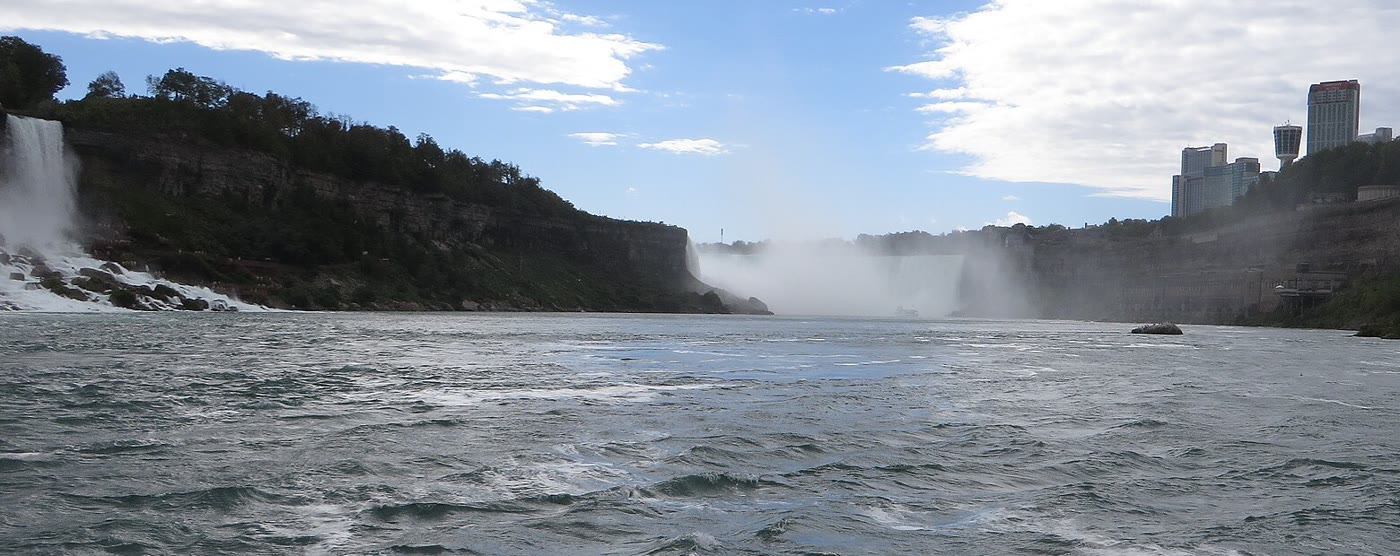
\includegraphics[width=\linewidth]{images/book5/b3-niagara-gorge.jpg}

{\scriptsize La garganta de Niágara, mirando aguas arriba hacia las cataratas de Herradura,
envueltas en su neblina, con las cataratas Americanas en el borde izquierdo. Fotografía de Ken Lund,
CC BY-SA 2.0 (recortada).}
\end{minipage}
\end{inthefield}
% ledger: ijc18:niagara, photo:b3-niagara-gorge


\section{Erosión glaciar}\label{sec:b3:quantitative-geomorphology:glacial}

Un glaciar que se desliza sobre su lecho (deslizamiento basal,
Capítulo~\ref{ch:b3:glaciology}) lo erosiona por abrasión, cuando los detritos que lleva retenidos en
el hielo raspan la roca, y por arranque, cuando arrastra bloques que se han aflojado por
las grietas. Ambos procesos escalan con la velocidad de deslizamiento.

\begin{definition}[Ley de erosión glaciar]\label{def:b3:quantitative-geomorphology:glacial}
Una \emph{ley de erosión glaciar}\index{ley de erosión glaciar} proporciona la tasa de
erosión del lecho de un glaciar como $E = K_G\,u_s^{\,l}$, donde $u_s$ es la
velocidad de deslizamiento, $K_G$ un coeficiente y $l$ un exponente.
\end{definition}

Los modelos de paisaje suelen tomar $l = 1$, aunque se emplean valores entre 1 y 2.
Una recopilación de 38 glaciares, cuyas tasas de erosión abarcan cinco órdenes de
magnitud, halló que la erosión se correlaciona con la velocidad de deslizamiento, con $l = 0.65$ y
$K_G = 10^{-4}$ para $E$ en metros al año: la erosión es más rápida bajo glaciares templados
alimentados por abundante nieve, que se deslizan rápido. Como el hielo es más grueso
y más veloz a lo largo del eje de un valle, el fondo se profundiza más que
los flancos, y el valle adquiere su forma en U.
% ledger: cook20:glacial

\begin{definition}[Sierra glaciar]\label{def:b3:quantitative-geomorphology:buzzsaw}
La \emph{sierra glaciar}\index{sierra glaciar} es el límite que imponen los glaciares a la
altura de una cordillera: allí donde la roca se eleva por encima de la altitud
a la que se forman los glaciares, estos la erosionan tan rápido como se eleva, sea cual sea
la tasa de levantamiento, de modo que las cumbres y la elevación media se agrupan en torno a esa altitud.
\end{definition}

\section{Tectónica y erosión}\label{sec:b3:quantitative-geomorphology:tectonics}

\begin{definition}[Estado estacionario topográfico]\label{def:b3:quantitative-geomorphology:steady-state}
Un paisaje se encuentra en \emph{estado estacionario topográfico}\index{estado estacionario topográfico}
cuando su tasa de erosión iguala en todas partes la tasa de levantamiento de la roca, de modo que
sus elevaciones no cambian aunque la roca pase a través de él.
\end{definition}

Las tasas medidas en intervalos de tiempo distintos permiten contrastar este estado. Los \omterm{def:b3:advanced-geochronology:cosmogenic}{nucleidos
cosmogénicos} en la arena de los ríos dan la tasa media de erosión de una cuenca durante el tiempo
necesario para eliminar una capa del orden de la longitud de atenuación de su
producción, unos \qty{55}{cm} de roca; los \omterm{def:b3:orogenic-wedges:thermochronology}{termocronómetros} y sus relaciones edad--altitud dan la
tasa de exhumación a lo largo de millones de años. Cuando ambas coinciden entre sí y con la
tasa de levantamiento, el paisaje probablemente está en \omterm{def:b3:quantitative-geomorphology:steady-profile}{estado estacionario}; cuando la
tasa a corto plazo es más rápida en el curso bajo que en la cabecera, un \omterm{def:b3:quantitative-geomorphology:knickpoint}{punto de ruptura de pendiente}
está pasando. Retirar roca también descarga la
litosfera, que se eleva en respuesta.
% ledger: zech04:exposure

\begin{definition}[Rebote isostático por erosión]\label{def:b3:quantitative-geomorphology:rebound}
El \emph{rebote isostático por erosión}\index{rebote isostático por erosión} es el ascenso de la
superficie rocosa de una región en equilibrio isostático como respuesta a la masa
eliminada por la erosión.
\end{definition}

\begin{proposition}[Las cumbres se elevan a medida que se profundizan los valles]\label{prop:b3:quantitative-geomorphology:rebound}
En la isostasia de Airy, con una corteza de densidad $\rho_c$ sobre un manto de densidad
$\rho_m$, la eliminación de un espesor medio $\bar e$ de corteza en una región eleva
toda la región en $(\rho_c/\rho_m)\,\bar e$. Si la erosión se limita
a los valles, las cumbres no erosionadas se elevan esa cantidad, mientras que la
superficie media desciende solo $(1 - \rho_c/\rho_m)\,\bar e$.
\end{proposition}

\begin{proof}
La compensación exige que la masa de cada columna por encima de una profundidad fija se mantenga
igual. Al retirar un espesor $\bar e$ de corteza, promediado sobre el área
de compensación, la masa por unidad de área disminuye en $\rho_c \bar e$;
para reponerla, el manto debe fluir hacia dentro a profundidad, elevando la base de la
columna, y todo lo que hay encima, en $\delta$ con $\rho_m \delta = \rho_c \bar
e$. Una cumbre que no perdió roca se eleva en $\delta$; la superficie media pierde
$\bar e$ y gana $\delta$.
\end{proof}

La densidad ponderada por espesor de la corteza del modelo de Tierra de referencia es
\qty{2.72}{g/cm^3} y la del manto bajo su Moho \qty{3.38}{g/cm^3},
una razón de 0.80: por cada cien metros de roca erosionada, la superficie media
pierde solo veinte. La incisión profunda de una meseta antigua puede así elevar
sus cumbres incluso mientras la meseta se desgasta.
% ledger: prem:crust-mantle-ratio

\begin{omfigure}
\begin{tikzpicture}[x=0.6cm, y=0.6cm, font=\scriptsize]
\begin{scope}
\fill[omDef!12] (0,0) rectangle (8,4);
\draw[thick] (0,4) -- (8,4);
\draw[densely dashed] (0,0) -- (8,0);
\node[anchor=north] at (4,-0.1) {base de la corteza};
\node at (4,2) {corteza $\rho_c$};
\node at (4,-1.2) {manto $\rho_m$};
\node[anchor=south] at (4,4.1) {antes};
\end{scope}
\begin{scope}[xshift=6.2cm]
\fill[omDef!12] (0,0.8) -- (0,4.8) -- (1.4,4.8) -- (2.0,2.4) -- (2.6,4.8) -- (5.4,4.8) -- (6.0,2.4) -- (6.6,4.8) -- (8,4.8) -- (8,0.8) -- cycle;
\draw[thick] (0,4.8) -- (1.4,4.8) -- (2.0,2.4) -- (2.6,4.8) -- (5.4,4.8) -- (6.0,2.4) -- (6.6,4.8) -- (8,4.8);
\draw[black!50, densely dashed] (0,4) -- (8,4);
\draw[densely dashed] (0,0.8) -- (8,0.8);
\draw[densely dashed, black!40] (0,0) -- (8,0);
\draw[<->, omThm] (8.3,4.05) -- (8.3,4.75) node[midway, right] {$\delta$};
\draw[<->, omThm] (8.3,0.05) -- (8.3,0.75) node[midway, right] {$\delta$};
\node[anchor=west, font=\scriptsize] at (8.1,2.4) {$\delta = (\rho_c/\rho_m)\,\bar e$};
\node[anchor=south] at (4,5.0) {tras la incisión de los valles};
\node[anchor=north] at (2.0,2.3) {valle};
\end{scope}
\end{tikzpicture}

\par\smallskip{\small \omterm{def:b3:quantitative-geomorphology:rebound}{Rebote isostático por erosión}, esquema. Excavar los
valles elimina un espesor medio $\bar e$ de corteza; la columna se eleva
$\delta = (\rho_c/\rho_m)\bar e$ en su base y en sus cumbres no erosionadas
(la línea gris discontinua es la superficie antigua).}\label{fig:b3:quantitative-geomorphology:rebound}
\end{omfigure}

\section{Ejercicios}

\begin{exercise}[$\star$]\label{exo:b3:quantitative-geomorphology:1}
Un escarpe litoral de desplazamiento \qty{4}{m} ($a = \qty{2}{m}$) se asienta sobre
una pendiente de campo lejano de 0.04, y su gradiente más pronunciado es ahora 0.30. Calcúlese
$\kappa t$, y después la edad del escarpe con $\kappa = \qty{5e-3}{m^2/yr}$.
\end{exercise}
% ledger: whipple04:scarp-erf, whipple04:scarp-kappa

\begin{exercise}[$\star$]\label{exo:b3:quantitative-geomorphology:2}
Un estudio lidar proporciona una curvatura en la cima de \qty{-0.012}{m^{-1}} en una cresta
de difusividad \qty{4e-3}{m^2/yr}. Calcúlese su tasa de erosión en
\unit{mm/yr}, y el relieve entre su cresta y los cauces
situados a \qty{80}{m}, suponiendo \omterm{def:b3:quantitative-geomorphology:steady-profile}{estado estacionario}.
\end{exercise}

\begin{exercise}[$\star$]\label{exo:b3:quantitative-geomorphology:3}
Con $m = 0.5$, $n = 1$ y $K = \qty{2e-6}{yr^{-1}}$, calcúlese la
tasa de incisión de un río que drena \qty{25}{km^2} con un gradiente de 0.01.
¿Cuáles son las unidades de $K$ para $m$ y $n$ generales?
\end{exercise}

\begin{exercise}[$\star$]\label{exo:b3:quantitative-geomorphology:4}
Tres ríos muestran \omterm{def:b3:quantitative-geomorphology:knickpoint}{puntos de ruptura de pendiente}: (a) donde un estrato de arenisca atraviesa un valle
excavado en lutita; (b) donde un río cruza una falla normal activa desde el
bloque inferior al bloque superior; (c) en cada río de una cuenca, todos a
una misma altitud, a pocos kilómetros por encima de una costa que se elevó en
un terremoto. ¿Cuáles están fijos y cuáles migrarán?
\end{exercise}

\begin{exercise}[$\star\star$]\label{exo:b3:quantitative-geomorphology:5}
Para $m = 1$ y $n = 2$, calcúlense $\theta$ y el gradiente de \omterm{def:b3:quantitative-geomorphology:steady-profile}{estado estacionario} donde $A =
\qty{10}{km^2}$, con $U = \qty{0.1}{mm/yr}$ y $K = 10^{-9}$ en metros y
años.
¿En qué factor cambia la pendiente si $U$ se duplica? Compárese con $n =
1$.
\end{exercise}

\begin{exercise}[$\star\star$]\label{exo:b3:quantitative-geomorphology:6}
El área de drenaje de un río crece con la distancia $d$ a su divisoria como $A =
c\,d^{h}$. Demuéstrese que, medido aguas arriba desde su desembocadura en $d = L$,
\[
\chi(d) = \frac{A_0^{\theta}}{c^{\theta}}\,\frac{L^{p} - d^{p}}{p},
\qquad p = 1 - h\theta ,
\]
y calcúlese para $c = 2$ (SI), $h = 1.8$, $\theta = 0.45$, $A_0 =
\qty{1}{km^2}$, $L = \qty{20}{km}$ y $d = \qty{5}{km}$.
\end{exercise}

\begin{exercise}[$\star\star$]\label{exo:b3:quantitative-geomorphology:7}
Con $n = 1$, $m = 0.5$ y $K = \qty{2e-6}{yr^{-1}}$, calcúlese la
celeridad de un \omterm{def:b3:quantitative-geomorphology:knickpoint}{punto de ruptura de pendiente} donde $A = \qty{100}{km^2}$, en m/kyr, y el
tiempo que tardaría en recorrer \qty{5}{km} a esa velocidad. ¿Por qué
en realidad tarda más?
\end{exercise}

\begin{exercise}[$\star\star$]\label{exo:b3:quantitative-geomorphology:8}
Valles de \qty{600}{m} de profundidad, que ocupan de media el \qty{40}{\percent} del
área de una meseta, se excavan en ella. Con $\rho_c/\rho_m = 0.80$, calcúlense
el espesor medio erosionado, la elevación de las cumbres y el cambio de la
altitud media.
\end{exercise}
% ledger: prem:crust-mantle-ratio

\begin{exercise}[$\star\star$]\label{exo:b3:quantitative-geomorphology:9}
Una \omterm{def:b3:quantitative-geomorphology:soil-production}{función de producción de suelo} tiene $P_0 = \qty{0.3}{mm/yr}$ y $h_0 =
\qty{0.5}{m}$. Calcúlese el espesor de suelo en \omterm{def:b3:quantitative-geomorphology:steady-profile}{estado estacionario} para una erosión de
\qty{0.05}{mm/yr} y de \qty{0.2}{mm/yr}. ¿Qué ocurre a
\qty{0.4}{mm/yr}?
\end{exercise}

\begin{exercise}[$\star\star\star$]\label{exo:b3:quantitative-geomorphology:10}
Una colina en \omterm{def:b3:quantitative-geomorphology:steady-profile}{estado estacionario} se erosiona a $E = \qty{0.1}{mm/yr}$ con $\kappa =
\qty{5e-3}{m^2/yr}$ y la ley no lineal de la \omterm{def:b3:quantitative-geomorphology:critical}{pendiente crítica de ladera}, tomando
$S_c = 1.2$ para el ejercicio. Demuéstrese que el flujo a una distancia $x$ de la
divisoria es $E x$, resuélvase para el gradiente y calcúlese en 20, 50, 100 y
\qty{200}{m}. Compárese con la difusión lineal y descríbase la forma de la
colina.
\end{exercise}

\begin{exercise}[$\star\star\star$]\label{exo:b3:quantitative-geomorphology:11}
Demuéstrese que el tiempo de respuesta de una red fluvial a un cambio en su desembocadura,
para $n = 1$, es $\chi_h/(K A_0^m)$, donde $\chi_h$ es el valor máximo de
$\chi$ en una cabecera de cauce. Calcúlese para el río de tierras altas de las figuras
($A_0 = \qty{1}{km^2}$, $m = 0.5$, $K = \qty{e-6}{yr^{-1}}$), primero para su
tronco principal solo, cuya cabecera está en $\chi = \qty{5464}{m}$, y después para la red,
cuya cabecera más alta, en el afluente 1, está en $\chi = \qty{7237}{m}$.
\end{exercise}

\begin{exercise}[$\star\star\star$]\label{exo:b3:quantitative-geomorphology:12}
En una red con $n = 1$ y $U$ uniforme, un afluente fluye sobre una roca dos veces
más erosionable que el resto ($2K$) aguas arriba de su confluencia, en $\chi_j$. Demuéstrese que
su línea de \omterm{def:b3:quantitative-geomorphology:steady-profile}{estado estacionario} en el plano $(\chi, z)$ tiene la mitad de la pendiente del
tronco principal por encima de $\chi_j$, y que un punto de ruptura nacido en la desembocadura alcanza,
en el momento en que el punto de ruptura del tronco está en $\chi_k > \chi_j$, el punto
de $\chi = \chi_j + 2(\chi_k - \chi_j)$ de ese afluente.
\end{exercise}

\section{Problema: la cascada del río Varden}

\begin{problem}[{Problema de fin de semana --- el perfil, la pendiente y la erodibilidad
de un río de tierras altas inventado, y la edad de su cascada}]
\label{pb:b3:quantitative-geomorphology:1}
Al oeste de las colinas Varden, el río drena una zona alta de esquistos antes de
entrar en el mapa por su borde oeste, a una altitud de \qty{170}{m}. Aguas arriba de ese punto,
su desembocadura, el tronco tiene \qty{12}{km} de longitud desde su divisoria,
con un área de drenaje $A = 4.5\,d^{1.7}$ (\unit{m^2}, $d$ en metros desde la
divisoria) y una cabecera de cauce en $d = \qty{300}{m}$. Tómese como tasa de levantamiento de la roca
la tasa de denudación de la cuenca del río Varden, obtenida a partir de sus cargas
en el volumen de primer año, \qty{43}{m/Myr}. Tómese $n = 1$ y el área de referencia $A_0 = \qty{1}{km^2}$.
Una cascada de \qty{25}{m} de altura se encuentra en el tronco, a \qty{4.60}{km} aguas arriba de
la desembocadura. Todos los valores son inventados.

\medskip\noindent\textbf{Parte I --- El perfil.}
\begin{enumerate}
\item Calcúlese el área de drenaje en la desembocadura y en la cabecera del cauce.
\item Gradientes medidos en tramos de \qty{200}{m}, alejados de la
  cascada:

  \smallskip
  {\small\begin{tabular}{l*{6}{c}}
  $A$ (\unit{km^2}) & 0.388 & 0.587 & 0.888 & 1.345 & 2.036 & 3.082 \\
  $S$ & 0.06641 & 0.05026 & 0.04888 & 0.03322 & 0.03688 & 0.02688 \\[2pt]
  $A$ (\unit{km^2}) & 4.665 & 7.061 & 10.69 & 16.18 & 24.49 & 37.08 \\
  $S$ & 0.01921 & 0.01713 & 0.01545 & 0.01419 & 0.007922 & 0.007855
  \end{tabular}}

  \smallskip
  Estímese el \omterm{def:b3:quantitative-geomorphology:indices}{índice de concavidad} a partir del primer y del último punto.
\item La pendiente de mínimos cuadrados de $\log S$ frente a $\log A$ es $-0.466$.
  ¿Es compatible con $\theta = 0.5$?
\item Con $\theta_{\mathrm{ref}} = 0.5$, calcúlese $k_{sn} = S A^{0.5}$ ($A$ en
  \unit{m^2}) para el primer y el último punto, y dígase qué representa la media
  geométrica de los doce valores, \qty{45.1}{m}.
\item ¿Por qué se dispersan mucho más los gradientes que las elevaciones?
\item Usando la fórmula del ejercicio de chi, calcúlese $\chi$ en $d =
  \qty{9.00}{km}$, un punto aguas abajo de la cascada.
\end{enumerate}

\medskip\noindent\textbf{Parte II --- Pendiente y erosionabilidad.}
\begin{enumerate}[resume]
\item El río se encuentra a \qty{193.4}{m} en $d = \qty{9.00}{km}$. Calcúlese la
  pendiente del gráfico de chi aguas abajo de la cascada y el \omterm{def:b3:quantitative-geomorphology:indices}{índice de pendiente del cauce} $k_{sn}$.
\item ¿En cuál de las dos estimaciones de $k_{sn}$, esta o la de pendiente--área,
  confiaría más, y por qué?
\item Suponiendo \omterm{def:b3:quantitative-geomorphology:steady-profile}{estado estacionario} aguas abajo de la cascada, calcúlese $K$ a partir de la
  tasa de levantamiento.
\item Compruébese que la tasa de incisión en la desembocadura, cuyo gradiente es
  0.00691, es igual a la tasa de levantamiento.
\item Calcúlese la celeridad de un \omterm{def:b3:quantitative-geomorphology:knickpoint}{punto de ruptura de pendiente} en la desembocadura y en la
  cascada, en m/kyr.
\item Calcúlese la elevación de la cabecera del cauce en el perfil estacionario, y el
  relieve del tronco.
\end{enumerate}

\medskip\noindent\textbf{Parte III --- La cascada.}
\begin{enumerate}[resume]
\item ¿Por qué, con $n = 1$, la cascada ha mantenido la altura de la caída
  del \omterm{def:b3:quantitative-geomorphology:knickpoint}{nivel de base}?
\item Calcúlese $\chi$ en la cascada.
\item Calcúlese el tiempo que tardó el \omterm{def:b3:quantitative-geomorphology:knickpoint}{punto de ruptura de pendiente} desde la
  desembocadura hasta su posición actual.
\item ¿Dónde estará dentro de \qty{300}{kyr}?
\item El afluente 3 se une al tronco a \qty{2.5}{km} aguas arriba de la desembocadura; tiene
  \qty{5}{km} de longitud, con $A = 1.5\,s^{1.7}$ ($s$ desde su propia divisoria).
  ¿Dónde debería estar su cascada?
\item Los afluentes 1 y 2 se unen al tronco a 8 y \qty{5}{km} aguas arriba de la
  desembocadura. Explíquese por qué no tienen cascada.
\end{enumerate}

\medskip\noindent\textbf{Parte IV --- Las laderas y la edad.}
\begin{enumerate}[resume]
\item Un levantamiento con lidar por encima de la cascada proporciona una curvatura en la cima de
  \qty{-0.0086}{m^{-1}}. Con $\kappa = \qty{5e-3}{m^2/yr}$, calcúlese la
  tasa de erosión y compárese con la tasa de levantamiento.
\item Las laderas tienen unos \qty{150}{m} de longitud. Compárese su tiempo de respuesta
  $L^2/\kappa$ con la edad obtenida en la Parte III.
\item Descríbanse las laderas aguas abajo de la cascada en la actualidad, y
  cómo cambiarán.
\item La tasa de levantamiento se conoce con un margen de \qty{20}{\percent}. Dése el intervalo de la
  edad.
\item ¿Cómo habría evolucionado la cascada si $n$ fuese 2?
\item Dése la edad de la caída del \omterm{def:b3:quantitative-geomorphology:knickpoint}{nivel de base}.
\end{enumerate}
\end{problem}
% ledger: whipple04:steepness, whipple04:scarp-kappa
